\documentclass[usenames,dvipsnames]{beamer}
\usepackage{../../shared/styles/custom}
\usepackage{../../shared/styles/conventions}

\usepackage{color, colortbl}
\usepackage{tikz}
\usetikzlibrary{shapes.geometric, arrows, positioning, calc}
\usepackage{array}
\usepackage{multirow}
\usepackage{booktabs}

% Define custom colors
\definecolor{lightblue}{RGB}{173,216,230}
\definecolor{lightgreen}{RGB}{144,238,144}
\definecolor{lightyellow}{RGB}{255,255,224}
\definecolor{lightpink}{RGB}{255,182,193}

\title{Next Token Generation}
\date{\today}
\author{Nipun Batra}
\institute{IIT Gandhinagar}

\begin{document}
\maketitle

\begin{frame}\vspace{0.5cm}
\begin{center}
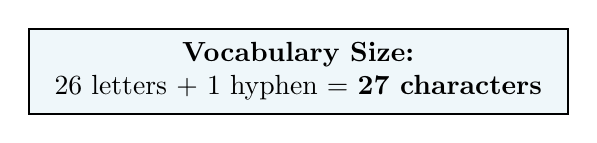
\begin{tikzpicture}
\node[draw, rectangle, thick, fill=lightblue!20] at (0,0) {
\begin{tabular}{c}
\textbf{Vocabulary Size:} \\
26 letters + 1 hyphen = \textbf{27 characters}
\end{tabular}
};
\end{tikzpicture}
\end{center}
\end{frame}

\section{Training Data Generation}

\begin{frame}\vspace{0.3cm}
\begin{center}
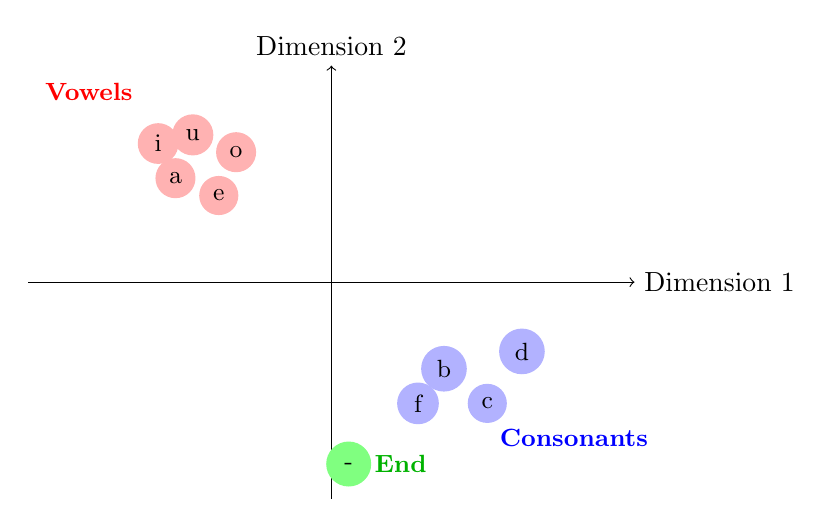
\begin{tikzpicture}[scale=1.1]
% Axes with better spacing
\draw[->] (-3.5,0) -- (3.5,0) node[right] {Dimension 1};
\draw[->] (0,-2.5) -- (0,2.5) node[above] {Dimension 2};

% Vowels cluster - better spaced
\node[circle, fill=red!30, inner sep=3pt] at (-1.8, 1.2) {\small a};
\node[circle, fill=red!30, inner sep=3pt] at (-1.3, 1.0) {\small e};
\node[circle, fill=red!30, inner sep=3pt] at (-2.0, 1.6) {\small i};
\node[circle, fill=red!30, inner sep=3pt] at (-1.1, 1.5) {\small o};
\node[circle, fill=red!30, inner sep=3pt] at (-1.6, 1.7) {\small u};

% Consonants cluster - better spaced
\node[circle, fill=blue!30, inner sep=3pt] at (1.3, -1.0) {\small b};
\node[circle, fill=blue!30, inner sep=3pt] at (1.8, -1.4) {\small c};
\node[circle, fill=blue!30, inner sep=3pt] at (2.2, -0.8) {\small d};
\node[circle, fill=blue!30, inner sep=3pt] at (1.0, -1.4) {\small f};

% Special character
\node[circle, fill=green!50, inner sep=4pt] at (0.2, -2.1) {\small -};

% Labels with better positioning
\node[color=red, font=\small\bfseries] at (-2.8, 2.2) {Vowels};
\node[color=blue, font=\small\bfseries] at (2.8, -1.8) {Consonants};
\node[color=green!70!black, font=\small\bfseries] at (0.8, -2.1) {End};
\end{tikzpicture}
\end{center}
\end{frame}

\begin{frame}{Word2Vec Analogy Example}
\begin{center}
\textbf{Classic Word2Vec Relationship}
\vspace{0.5cm}

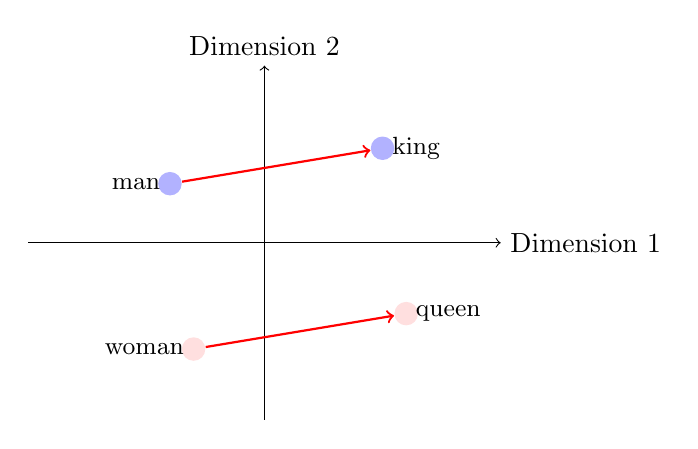
\begin{tikzpicture}[scale=1.5]
% Vector space
\draw[->] (-2,0) -- (2,0) node[right] {Dimension 1};
\draw[->] (0,-1.5) -- (0,1.5) node[above] {Dimension 2};

% Points
\node[circle, fill=blue!30, inner sep=3pt] (king) at (1, 0.8) {};
\node[right] at (king) {\small king};

\node[circle, fill=pink!50, inner sep=3pt] (queen) at (1.2, -0.6) {};
\node[right] at (queen) {\small queen};

\node[circle, fill=blue!30, inner sep=3pt] (man) at (-0.8, 0.5) {};
\node[left] at (man) {\small man};

\node[circle, fill=pink!50, inner sep=3pt] (woman) at (-0.6, -0.9) {};
\node[left] at (woman) {\small woman};

% Arrows
\draw[->, thick, red] (man) -- (king);
\draw[->, thick, red] (woman) -- (queen);
\end{tikzpicture}

\vspace{0.5cm}
\textbf{Relationship:} queen $\approx$ king - man + woman
\end{center}
\end{frame}

\begin{frame}{Analogy with Emotions}
\begin{center}
\textbf{Emotional Expression Analogy}
\vspace{0.5cm}

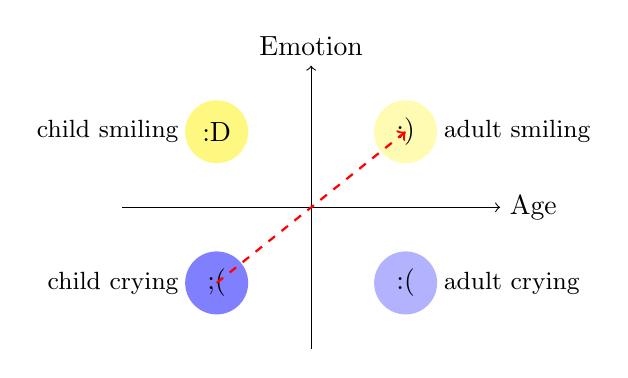
\begin{tikzpicture}[scale=1.2]
% Vector space
\draw[->] (-2,0) -- (2,0) node[right] {Age};
\draw[->] (0,-1.5) -- (0,1.5) node[above] {Emotion};

% Emotional representations using circles with symbols
\node[circle, fill=yellow!30, minimum size=0.8cm] at (1, 0.8) {:)};
\node[right] at (1.3, 0.8) {\small adult smiling};

\node[circle, fill=blue!30, minimum size=0.8cm] at (1, -0.8) {:(};
\node[right] at (1.3, -0.8) {\small adult crying};

\node[circle, fill=yellow!50, minimum size=0.8cm] at (-1, 0.8) {:D};
\node[left] at (-1.3, 0.8) {\small child smiling};

\node[circle, fill=blue!50, minimum size=0.8cm] at (-1, -0.8) {;(};
\node[left] at (-1.3, -0.8) {\small child crying};

% Arrows showing relationship
\draw[->, thick, red, dashed] (-1, -0.8) -- (1, 0.8);
\end{tikzpicture}

\vspace{0.5cm}
\textbf{Relationship:} child crying = child smiling + adult crying - adult smiling
\end{center}
\end{frame}

\section{Embedding Architecture}

\begin{frame}{Embedding Matrix/Table Concept}
\begin{center}
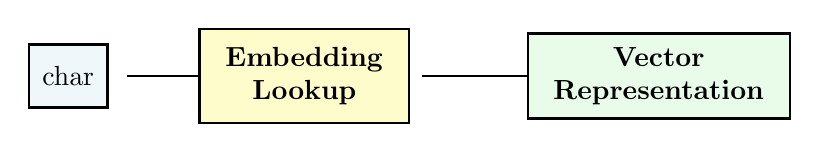
\begin{tikzpicture}[scale=1.5]
% Input character
\node[draw, rectangle, thick, minimum width=1cm, minimum height=0.8cm, fill=lightblue!20] at (-2,0) {char};

% Arrow
\draw[->, thick] (-1.5, 0) -- (-0.5, 0);

% Embedding block
\node[draw, rectangle, thick, minimum width=2cm, minimum height=1.2cm, fill=yellow!20] at (0,0) {
\begin{tabular}{c}
\textbf{Embedding} \\
\textbf{Lookup}
\end{tabular}
};

% Arrow
\draw[->, thick] (1, 0) -- (2, 0);

% Output vector
\node[draw, rectangle, thick, minimum width=1.5cm, minimum height=0.8cm, fill=lightgreen!20] at (3,0) {
\begin{tabular}{c}
\textbf{Vector} \\
\textbf{Representation}
\end{tabular}
};
\end{tikzpicture}
\end{center}

\vspace{1cm}
\begin{center}
\textbf{Process:} Character $\rightarrow$ Lookup in Embedding Table $\rightarrow$ Dense Vector
\end{center}
\end{frame}

\begin{frame}{Embedding Table Structure}
\begin{center}
\textbf{27 × K Embedding Matrix}
\vspace{0.3cm}

\begin{tabular}{|c|c|c|c|c|}
\hline
\textbf{Char} & \textbf{D1} & \textbf{D2} & \textbf{...} & \textbf{DK} \\
\hline
a & 0.2 & -0.1 & ... & 0.8 \\
b & -0.3 & 0.5 & ... & -0.2 \\
c & 0.1 & 0.3 & ... & 0.4 \\
$\vdots$ & $\vdots$ & $\vdots$ & $\ddots$ & $\vdots$ \\
z & 0.7 & -0.4 & ... & 0.1 \\
- & 0.0 & 0.9 & ... & -0.5 \\
\hline
\end{tabular}
\end{center}

\vspace{0.3cm}
\begin{alertblock}{Key Point}
Each character maps to a K-dimensional vector.
\end{alertblock}
\end{frame}

\begin{frame}{Learnable Parameters}
\begin{itemize}
\item \textbf{Embedding Matrix:} 27 × K parameters
\begin{itemize}
\item Initially random
\pause
\item Updated during training via backpropagation
\item Learns meaningful character representations
\end{itemize}

\item \textbf{Neural Network Weights:} MLP parameters
\begin{itemize}
\item Transform concatenated embeddings to output
\item Learn classification patterns
\end{itemize}

\item \textbf{Total Learnable Parameters:}
\begin{itemize}
\item Embedding: 27 × K
\item MLP: (context\_size × K) → hidden → ... → 27
\end{itemize}
\end{itemize}
\end{frame}

\section{Neural Network Architecture}

\begin{frame}{Example: 2D Embeddings for ``abi''}
\begin{center}
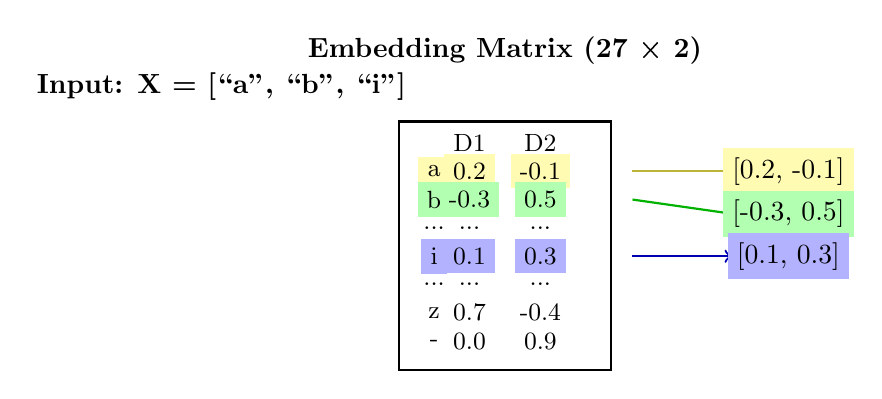
\begin{tikzpicture}[scale=0.9]
% Input vector
\node at (-4, 3) {\textbf{Input: X = [``a'', ``b'', ``i'']}};

% Embedding matrix
\node at (0, 3.5) {\textbf{Embedding Matrix (27 × 2)}};
\begin{scope}[shift={(0,0)}]
\draw[thick] (-1.5, 2.5) rectangle (1.5, -1);

% Headers
\node at (-0.5, 2.2) {\small D1};
\node at (0.5, 2.2) {\small D2};

% Character rows with colors
\node[fill=yellow!30] at (-1, 1.8) {\small a};
\node[fill=yellow!30] at (-0.5, 1.8) {\small 0.2};
\node[fill=yellow!30] at (0.5, 1.8) {\small -0.1};

\node[fill=green!30] at (-1, 1.4) {\small b};
\node[fill=green!30] at (-0.5, 1.4) {\small -0.3};
\node[fill=green!30] at (0.5, 1.4) {\small 0.5};

% Dots
\node at (-1, 1.0) {\small ...};
\node at (-0.5, 1.0) {\small ...};
\node at (0.5, 1.0) {\small ...};

\node[fill=blue!30] at (-1, 0.6) {\small i};
\node[fill=blue!30] at (-0.5, 0.6) {\small 0.1};
\node[fill=blue!30] at (0.5, 0.6) {\small 0.3};

% More dots
\node at (-1, 0.2) {\small ...};
\node at (-0.5, 0.2) {\small ...};
\node at (0.5, 0.2) {\small ...};

\node at (-1, -0.2) {\small z};
\node at (-0.5, -0.2) {\small 0.7};
\node at (0.5, -0.2) {\small -0.4};

\node at (-1, -0.6) {\small -};
\node at (-0.5, -0.6) {\small 0.0};
\node at (0.5, -0.6) {\small 0.9};
\end{scope}

% Arrows and extracted vectors
\draw[->, thick, yellow!70!black] (1.8, 1.8) -- (3.2, 1.8);
\node[fill=yellow!30] at (4, 1.8) {[0.2, -0.1]};

\draw[->, thick, green!70!black] (1.8, 1.4) -- (3.2, 1.2);
\node[fill=green!30] at (4, 1.2) {[-0.3, 0.5]};

\draw[->, thick, blue!70!black] (1.8, 0.6) -- (3.2, 0.6);
\node[fill=blue!30] at (4, 0.6) {[0.1, 0.3]};
\end{tikzpicture}
\end{center}
\end{frame}

\begin{frame}{Concatenate the Embeddings}
\begin{center}
\textbf{Feature Vector Construction}
\vspace{0.3cm}

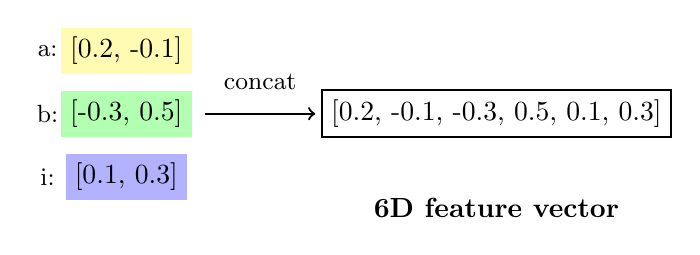
\begin{tikzpicture}[scale=1.0]
% Input embeddings with better spacing
\node[fill=yellow!30, minimum width=1.3cm, minimum height=0.5cm] at (-2.2, 0.8) {[0.2, -0.1]};
\node at (-3.2, 0.8) {\small a:};

\node[fill=green!30, minimum width=1.3cm, minimum height=0.5cm] at (-2.2, 0) {[-0.3, 0.5]};
\node at (-3.2, 0) {\small b:};

\node[fill=blue!30, minimum width=1.3cm, minimum height=0.5cm] at (-2.2, -0.8) {[0.1, 0.3]};
\node at (-3.2, -0.8) {\small i:};

% Arrow with better positioning
\draw[->, thick] (-1.2, 0) -- (0.2, 0);
\node at (-0.5, 0.4) {\small concat};

% Result with adjusted width
\node[draw, rectangle, thick, minimum width=3.5cm, minimum height=0.6cm] at (2.5, 0) {
[0.2, -0.1, -0.3, 0.5, 0.1, 0.3]
};

\node at (2.5, -1.2) {\textbf{6D feature vector}};
\end{tikzpicture}
\end{center}

\vspace{0.3cm}
\begin{alertblock}{Result}
3 chars × 2D embeddings = 6D input to neural network
\end{alertblock}
\end{frame}

\begin{frame}{Multi-Layer Perceptron Architecture}
\begin{center}
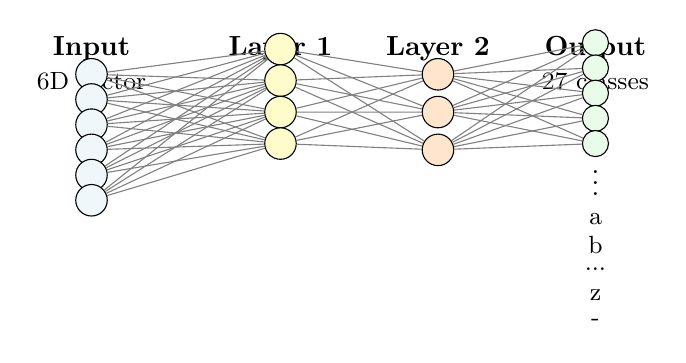
\begin{tikzpicture}[scale=0.8]
% Input layer
\node at (-4, 3) {\textbf{Input}};
\node at (-4, 2.5) {\small 6D vector};
\foreach \i in {1,2,3,4,5,6} {
    \node[circle, draw, fill=lightblue!20, minimum size=0.4cm] (input\i) at (-4, 3-\i*0.4) {};
}

% Hidden layer 1
\node at (-1, 3) {\textbf{Layer 1}};
\foreach \i in {1,2,3,4} {
    \node[circle, draw, fill=yellow!20, minimum size=0.4cm] (hidden1\i) at (-1, 3.5-\i*0.5) {};
}

% Hidden layer 2
\node at (1.5, 3) {\textbf{Layer 2}};
\foreach \i in {1,2,3} {
    \node[circle, draw, fill=orange!20, minimum size=0.4cm] (hidden2\i) at (1.5, 3.2-\i*0.6) {};
}

% Output layer
\node at (4, 3) {\textbf{Output}};
\node at (4, 2.5) {\small 27 classes};
\foreach \i in {1,2,3,4,5} {
    \node[circle, draw, fill=lightgreen!20, minimum size=0.3cm] (output\i) at (4, 3.5-\i*0.4) {};
}
\node at (4, 1) {\vdots};

% Connections (sample)
\foreach \i in {1,2,3,4,5,6} {
    \foreach \j in {1,2,3,4} {
        \draw[gray, thin] (input\i) -- (hidden1\j);
    }
}

\foreach \i in {1,2,3,4} {
    \foreach \j in {1,2,3} {
        \draw[gray, thin] (hidden1\i) -- (hidden2\j);
    }
}

\foreach \i in {1,2,3} {
    \foreach \j in {1,2,3,4,5} {
        \draw[gray, thin] (hidden2\i) -- (output\j);
    }
}

% Labels
\node at (4, 0.3) {\small a};
\node at (4, -0.1) {\small b};
\node at (4, -0.5) {\small ...};
\node at (4, -0.9) {\small z};
\node at (4, -1.3) {\small -};
\end{tikzpicture}
\end{center}
\end{frame}

\section{Training and Loss Function}

\begin{frame}{Training Objective}
\begin{itemize}
\item \textbf{Loss Function:} Cross-entropy loss for multi-class classification

\begin{equation}
\mathcal{L} = -\sum_{i=1}^{N} \sum_{c=1}^{27} y_{i,c} \log(\hat{y}_{i,c})
\end{equation}

\pause
\item \textbf{What we learn:}
\begin{enumerate}
\pause
\item \textbf{Embedding Matrix:} Character representations (27 × K parameters)
\pause
\item \textbf{MLP Weights:} Neural network parameters for classification
\end{enumerate}

\pause
\item \textbf{Training Process:}
\begin{enumerate}
\pause
\item Forward pass: Input → Embeddings → Concatenate → MLP → Probabilities
\item Compute cross-entropy loss
\item Backward pass: Update both embeddings and MLP weights
\pause
\item Repeat for all training examples
\end{enumerate}
\end{itemize}
\end{frame}

\section{Text Generation}

\begin{frame}{Sampling from the Learned Model}
\textbf{Test Input:} ``abi''

\vspace{0.5cm}
\begin{center}
\textbf{Predicted Probability Distribution}
\vspace{0.3cm}

\begin{tabular}{|c|c|c|c|}
\hline
\textbf{Next Char} & \textbf{Probability} & \textbf{Next Char} & \textbf{Probability} \\
\hline
a & 0.01 & n & 0.05 \\
b & 0.01 & o & 0.02 \\
c & 0.03 & p & 0.01 \\
d & \textcolor{red}{\textbf{0.60}} & q & 0.00 \\
e & 0.02 & r & 0.03 \\
f & 0.01 & s & 0.08 \\
... & ... & ... & ... \\
- & 0.05 & z & 0.01 \\
\hline
\end{tabular}
\end{center}

\vspace{0.5cm}
\begin{alertblock}{Most Likely Continuation}
``abi'' → ``abid'' (60% probability)
\end{alertblock}
\end{frame}

\begin{frame}{Generation Tree Structure}
\begin{center}
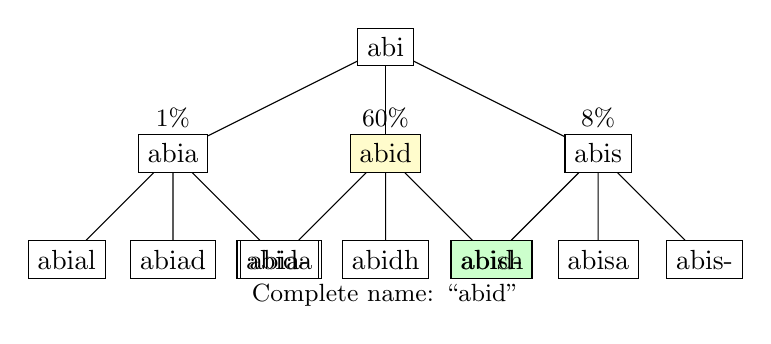
\begin{tikzpicture}[scale=0.9, level 1/.style={sibling distance=3cm}, level 2/.style={sibling distance=1.5cm}]
\node[draw, rectangle] {abi}
    child {
        node[draw, rectangle] {abia}
        child {node[draw, rectangle] {abial}}
        child {node[draw, rectangle] {abiad}}
        child {node[draw, rectangle] {abia-}}
    }
    child {
        node[draw, rectangle, fill=yellow!20] {abid}
        child {node[draw, rectangle] {abida}}
        child {node[draw, rectangle] {abidh}}
        child {node[draw, rectangle, fill=green!20] {abid-}}
    }
    child {
        node[draw, rectangle] {abis}
        child {node[draw, rectangle] {abish}}
        child {node[draw, rectangle] {abisa}}
        child {node[draw, rectangle] {abis-}}
    };

% Probabilities
\node at (-3, -1) {\small 1\%};
\node at (0, -1) {\small 60\%};
\node at (3, -1) {\small 8\%};

\node at (0, -3.5) {\small Complete name: ``abid''};
\end{tikzpicture}
\end{center}

\begin{center}
\textbf{Recursive Process:} Sample next character, append, repeat until end token
\end{center}
\end{frame}

\section{Temperature and Sampling Strategies}

\begin{frame}{Temperature in Softmax}
\begin{itemize}
\item \textbf{Standard Softmax:}
\begin{equation}
P(y_i) = \frac{e^{z_i}}{\sum_{j=1}^{27} e^{z_j}}
\end{equation}

\pause
\item \textbf{Temperature-scaled Softmax:}
\begin{equation}
P(y_i) = \frac{e^{z_i/T}}{\sum_{j=1}^{27} e^{z_j/T}}
\end{equation}

\pause
\item \textbf{Temperature Effects:}
\begin{itemize}
\item $T = 1$: Standard probabilities
\item $T \to 0$: More peaked (deterministic)
\pause
\item $T \to \infty$: More uniform (random)
\end{itemize}
\end{itemize}
\end{frame}

\begin{frame}{Temperature Variations}
\textbf{Context:} ``abi'' → Next character probabilities

\vspace{0.3cm}
\begin{center}
\begin{tabular}{|c|c|c|c|}
\hline
\textbf{Char} & \textbf{T=0.5} & \textbf{T=1.0} & \textbf{T=2.0} \\
 & \textbf{(Low)} & \textbf{(Default)} & \textbf{(High)} \\
\hline
a & 0.001 & 0.01 & 0.08 \\
d & \textbf{0.95} & \textbf{0.60} & \textbf{0.25} \\
s & 0.01 & 0.08 & 0.12 \\
h & 0.005 & 0.03 & 0.09 \\
- & 0.02 & 0.05 & 0.11 \\
others & 0.015 & 0.23 & 0.35 \\
\hline
\end{tabular}
\end{center}

\vspace{0.3cm}
\begin{itemize}
\item \textbf{Low T:} Conservative, predictable
\pause
\item \textbf{High T:} Creative, diverse
\end{itemize}
\end{frame}

\section{Summary and Applications}

\begin{frame}{Key Takeaways}
\begin{itemize}
\item \textbf{Core Idea:} Next token prediction as classification
\pause
\item \textbf{Representation Learning:} Character embeddings capture similarity
\pause
\item \textbf{Architecture:} Embeddings + MLP for sequence modeling
\pause
\item \textbf{Training:} Joint learning of embeddings and classifier weights
\pause
\item \textbf{Generation:} Autoregressive sampling with temperature control
\pause
\item \textbf{Applications:} Foundation for modern language models
\begin{itemize}
\item GPT models use the same principle
\item Scaled to words/subwords instead of characters
\pause
\item Transformer architecture instead of MLP
\item Billions of parameters instead of thousands
\end{itemize}
\end{itemize}
\end{frame}

\begin{frame}{From Character-Level to ChatGPT}
\begin{center}
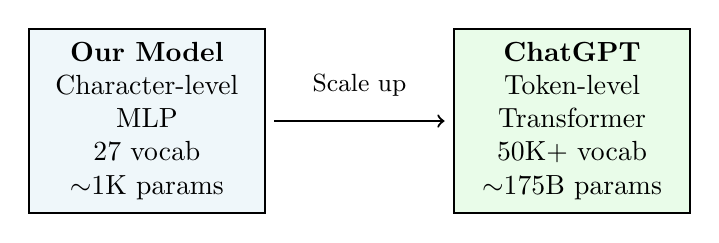
\begin{tikzpicture}[scale=0.9]
% Our model
\node[draw, rectangle, thick, fill=lightblue!20, minimum width=3cm, minimum height=1.5cm] at (-3, 0) {
\begin{tabular}{c}
\textbf{Our Model} \\
Character-level \\
MLP \\
27 vocab \\
$\sim$1K params
\end{tabular}
};

% Arrow
\draw[->, thick] (-1.2, 0) -- (1.2, 0);
\node at (0, 0.5) {\small Scale up};

% ChatGPT
\node[draw, rectangle, thick, fill=lightgreen!20, minimum width=3cm, minimum height=1.5cm] at (3, 0) {
\begin{tabular}{c}
\textbf{ChatGPT} \\
Token-level \\
Transformer \\
50K+ vocab \\
$\sim$175B params
\end{tabular}
};
\end{tikzpicture}
\end{center}

\vspace{0.5cm}
\begin{center}
\textbf{Same fundamental principle: Predict the next token!}
\end{center}
\end{frame}

\end{document}